\documentclass{article}
\usepackage[utf8]{inputenc}
\usepackage{hyperref}
\usepackage{standalone}
%\definecolor{linkcolour}{rgb}{0,0.2,0.6}
\usepackage{color}
\usepackage{xcolor} %for more colours to use in hyperref
\usepackage{graphicx}
\usepackage{float}
\usepackage{enumerate}
\graphicspath{{Images/}}
\definecolor{forestgreen}{rgb}{0.0, 0.5, 0.0}
\hypersetup{
    colorlinks=true, %set true if you want colored links
    linkcolor=forestgreen,
    citecolor={blue!50!black},
    urlcolor={blue!80!black}
    }
\usepackage{biblatex}

\addbibresource{ref.bib}

    
\usepackage{titlesec}

\setcounter{secnumdepth}{4}

\titleformat{\paragraph}
{\normalfont\normalsize\bfseries}{\theparagraph}{1em}{}
\titlespacing*{\paragraph}
{0pt}{3.25ex plus 1ex minus .2ex}{1.5ex plus .2ex}    

\title{Automated Evaluation of Programming Assignments \\ \vspace{0.5mm} \large\textit{Report}}
\author{Rishabh Manoj}
\date{\today}

\begin{document}

\maketitle
\section{Introduction}

The assessment of programming assignments places significant demands on the instructor’s time and other resources. This demand has led to the creation of automatic evaluation systems. Students are given programming assignments which are assessed using automatic program evaluation systems. These systems provide a possibility for the student to submit a solution, test it in some way and receive feedback. Such systems could also provide feedback for the teachers and evaluators.

One naive method which is commonly used is to manually create a set of test-cases that can be used to assess the solutions. While these are effective in identifying whether the solution is correct or not, this will not give an indication to how similar the student's solution is to the correct solution.

In this paper we come up with a method that will try to answer the above question.

\section{Definitions}

\subsection*{Symbolic Testing}
Symbolic testing is the one of the program analysis technique used for proving program correctness. This technique executes the programs using symbolic values instead of concrete input data and represents the program variables as symbolic expressions. Therefore, we are able to represent the output of the program as a function of symbolic values. The most widely used application of symbolic testing is the automated test case generation for proving program correctness.

\subsection*{Program Dependence Graph:} Program dependence graph (PDG) is a graphical representation of the source code of a program. Basic statements, like variable declarations, assignments, and procedure calls, are represented by program vertices in PDG’s. The data and control
dependencies between statements are represented by edges between program vertices
in PDG’s.\\

\subsection*{Graph Isomorphism}
A graph can have the different form which contains the same number of vertices, edges and vertices are connected in the same way are said to be isomorphic graphs. 

Formally, the graphs $G$ and $G'$ are isomorphic, then there exists a function $F: V(G) \to V(G')$ such that
\begin{enumerate}[i.]
  \item $f$ is a bijection.
  \item $f$ preserves adjacency of vertices. i.e. if the $(u,v) \in E(G)$ then $(f(u),f(v)) \in E(G')$
\end{enumerate}

\subsubsection*{$\gamma$ Isomorphism}
A graph $G$ is $\gamma$-isomorphic to $G^\prime$ if there exists a subgraph $S \subseteq G$ such that $S$ is
subgraph isomorphic to $G^\prime$ , and $\|S\| \geq \gamma \|G\|$, $\gamma \in$ (0,1). $\gamma$ is said to be the mature rate of isomorphic subgraphs. Initial $\gamma$ is set based on a belief on how much the subgraphs would be isomorphic. Value of $\gamma$ helps in pruning the search space for isomorphism. In other words, value of $\gamma$ would limit the number or vertices which would be subgraph isomorphic to the other graph.\\

\section{Proposed Method}

\subsection{Gold Standard Solutions:}
    In this module we separate the students' solution into Correct and Incorrect submissions.\\
    We are initially given all the students' solutions and one reference solution. Using the reference solution we automatically generate a set of test-cases that covers all the corner-case of the assignment and test it against the students' solution.  The solutions that passes all these test-cases are considered correct and the others are considered incorrect.
    
    We generate test-cases using Symbolic Testing \cite{Symbolic} tools like \textit{CREST}, \textit{API Sanity Check}, etc...

\subsection{Similarity Measure:}

    In this module, we calculate the similarity measure of the solutions with each other which is then later used for clustering.
    
    The central idea is to generate \textit{Program Dependence Graphs} \cite{PDG} for the solutions and check for sub-graph isomorphism between any two PDG's. If it is sub-graph isomorphic then based on the number of vertices mapped we calculate similarity. (No. of mapped vertices of Graph G1 / Total no. of vertices of Graph G2) [G1 sub-graph isomorphic to G2]

    PDG's are generated for each function. In this instance we assume that the datset contains only one function(main) and genearte PDG's for main functions. % A solution can have multiple functions with different function names for each of the solution. So to map PDG's properly, we generate a function call for the solution and do a simple linear mapping based on the positions of the function calls in the stack.Function call can be generated using the \textit{cflow} command in \textit{Linux}.
    
    We use \textit{frama-c} software to generate PDG's of the solution. This creates a DOT file for each of the function. To parse this, we use a DOT parser in python to get a grpah with vertices and nodes.We use $\gamma$-isomorphism method to calculate similarity. This$\gamma$-isomorphism method checks for sub-graph isomorphism between the PDG's and calculates similarity as mentioned above.  
    
\textit{Summary:}
\begin{itemize}
    \item Create PDG's using frama-c for each solution.
        \begin{itemize}
            \item DOT files for each function
            \item \textit{frama-c -pdg -pdg-dot filename c-programfile }.
        \end{itemize}
    \item Extract graph nodes and edges from DOT file using a DOT parser in python
    \item Calculate similarity measure using $\gamma$-isomorphism as mentioned above.
\end{itemize}

Output of this module is similarity measure of each pairs of solution ranging from $0$ to $1$ with $1$ being high similarity and 0 being no similarity.

\subsubsection{Implementation Details:}
    \begin{itemize}
        \item For each program, PDG has to be generated, we use \textit{frama-c} to generate a DOT file which contains the PDG.
        \item A DOTParser for python was used to extract nodes and edges from the DOT file. This was converted to a NetworkX graph in python.
        \item Sub graph isomorphism algorithm was used to calculate similarity.
    \end{itemize}
    
    \paragraph{Program Dependence Graph}
        
        \textit{Frama-c} is a set of interoperable program analyzers for C programs. We use \textit{Frama-c} to generate dependency graph in the form of DOT files for C programs. While it generates for most of the C programs it does not encompass the entire C language. 
        
        Frama-c (Flourine version) the stable release for Ubuntu 14.04 does not work with Variable Length array, the latest release of Frama-c (Phosphorous) while it works with single dimensional variable length array it doesnot for multi-dimensional arrays.
        
        The output of Frama-c's pdg generation is a DOT file which contains the nodes and edges of the PDG. DOT files are hard to interpret and contains unnecessary details, so a DOTParser was used to get only the nodes and edges. This was then used to instantiate a NetworkX graph (a python library for graphs) which was selected for it's vast graph related library.
        
    \paragraph{$\gamma$-isomorphism}
        
        We follow the algorithm provided in \cite{GPLAG} named $\gamma$-isomorphism as it uses a $\gamma$-filtering technique to eliminate certain graphs before performing subgraph isomorphism.
        
        Sub graph Isomorphism is an NP-Complete problem which means that there is no polynomial time solution. (Note that Graph Isomorphism is neither P nor NP-complete but it's generalisation(sub-graph isomorphism) is NP-complete). Over the years there have been many heuristic solutions that attempt to solve this for a specific set of graphs like the Glasgow algorithm \cite{Glasgow}, the VF2 algorithm \cite{VF} and recently the LAD filtering algorithm \cite{pathLAD}.
        
        Initially the \textit{VF2} algorithm was implemented as it was used in the algorithm mentioned in \cite{GPLAG}, we found that the algorithm is very time-consuming, while for graphs with very less nodes (in the range of 20 to 30) it calculates in seconds, the higher the vertex count (usually in the range of 100's which is the case for our dataset) it sometimes takes days to calculate!!
        
        Due to this the \textit{VF2} algorithm approach was abandoned and the latest development in sub graph isomorphism the LAD filtering approach was chosen. The latest variant, \textit{pathLAD} \cite{pathLAD}, was used. A time limit was set which can act as a threshold as to when the search can be discontinued.
        
        While the LAD algorithm works much faster than \textit{VF2}, there are still cases where sub-graphs could not be found within the time-limit. In some cases increasing the time-limit by a few seconds leads to solutions where it would not have found in the decreased time-space. This leads to drastic change in the output of the next phase.
        
\subsubsection{Suggestion:}
    Due to the unreliability of sub graph-isomorphism, find other similarity metrics like LOC, Function count, running time, memory usage, $\cdots$. Use a weighted average of these metrics to calculate a similarity index. This will lead to less dependence on graph isomorphism which will not drastically alter the overall output.

        \begin{figure}[H]
            \centering
                \centering
                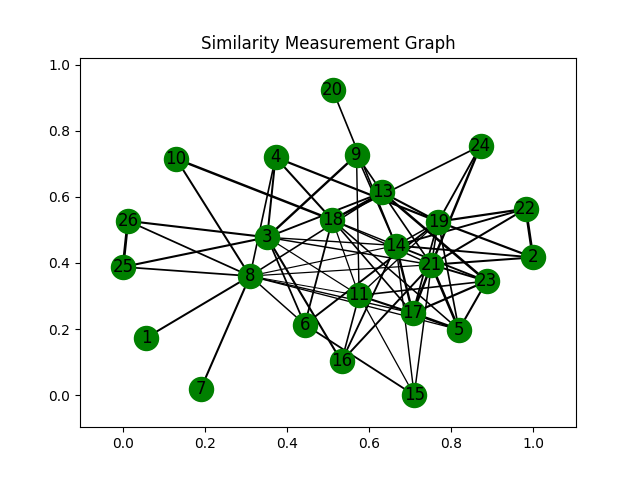
\includegraphics[height=1.2in]{Images/similarity_ensemble_1.png}
                \caption{Similarity Measure Ouput}
        \end{figure}

\subsection{Clustering:}

Graph clustering involves the task of dividing nodes into clusters, so that the edge density is higher within clusters as opposed to across clusters. Graph Clustering is a deeply studied problem as there are many use cases in biochemistry especially in clustering protein complexes. 

In this module we cluster similar solutions together to form some distinct types/methods/algorithms of solutions possible for the given problem.

The output from the above Similarity Measure module is considered as an edgelist in this module. The program files become the nodes and the similarity measure becomes the weights of the edge between them.

Using this graph, we start clustering. Idea is that nodes with edges whose similarity values are high will cluster together. 

The output of this module are clusters which contains program files.

\subsubsection{Implementation Details}
We use various clustering algorithms and compare their clusters to some human annotated clusters.
\paragraph{Louvain modularity}
    We use a method called Louvain modularity \cite{louvian} which is a greedy optimization method that appears to run in time O($n\log n$). In this method, first small communities are found by optimizing modularity locally on all nodes, then each small community is grouped into one node and the step is repeated.

    \textit{Observation:} Nodes within Clusters sometimes do not have high edge weights, while one node will be highly connected to everything the other nodes are not so strongly connected to each other node. 
    \textit{Possible explanation:} Since similarity values are calculated based on isomorphism which is NP-complete, the values for some pair of nodes might actually be high but since it cannot be found out in the stipulated time interval, the values are given zero. While clustering, if the neighbours of the nodes are highly similar then it is also highly likely that the node is similar to the rest of the others.
    
    For eg:
            For example there are 4 nodes 1,2,3 \& 4 if 1,2,3 are highly similar and 3,4 are also highly similar but the values for 1,4 and 2,4 are zero, it is highly possible that 1,4 and 2,4 are actually similar but the sub graph isomorphism could not find a solution within the given interval.
    
    \textit{Solution:} Add other parameters to include in similarity measurement. 
    
    
        \begin{figure}[H]
            \centering
                \centering
                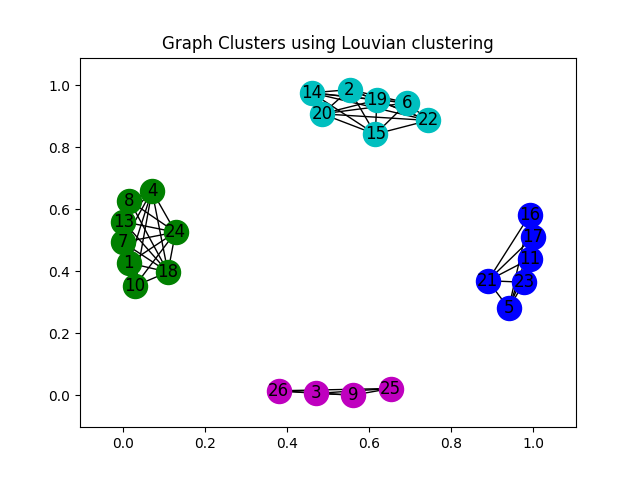
\includegraphics[scale=0.5]{Images/cluster_louvian_1.png}
                \caption{Louvian Clustering}
        \end{figure}
    
\paragraph{IPCA Clustering}
    Each point’s measure property can be transformed as the influence power against its neighbor points.\cite{ipca} If one point’s measure is larger, it would have more
influence power to attract its neighbor points, and its neighbors would have a trend to be absorbed by this point.

    \textit{Observation:} Within clusters, the similarity is high but same nodes are found in multiple clusters

        \begin{figure}[H]
            \centering
                \centering
                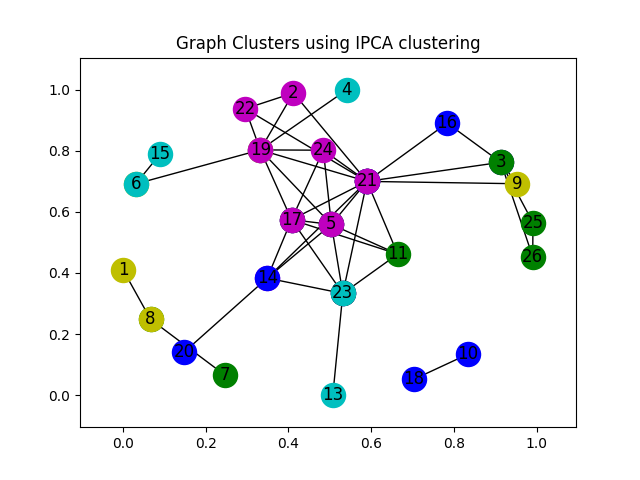
\includegraphics[scale=0.5]{Images/cluster_IPCA_1.png}
                \caption{IPCA Clustering}
        \end{figure}


%#TODO Put graphs images



\subsection{Marking Scheme:}
    
    This module is primarily for Incorrect solutions. The idea is to categorize the solution into the nearest cluster by calculating similarity measure with each of the Gold Standard solutions (Correct Solutions) and clustering into the nearest group.
    
    We get the similarity measure from the above module and find the most similar gold standard program and assign the cluster which the gold standard program is in.
    
    To assign a grade we use many factors like the no. of testcases it passed, the running time, amount of memory used, strength of similarity and intra-cluster distance, etc...
    


    
\printbibliography


\end{document}
